\chapter{One-to-many Relationships}
\label{chapter:representing-relationships}

One-to-many relationships
%such as those in an entity-relationship model,
are typically implemented in Java using the standard library collection classes.
Each object maintains a collection of the objects related to
it along a given relationship. Since one-to-many relationships are such an
important part of most data models, it is not uncommon for Java applications to
need hundreds of thousands, or even millions, of collections.
Therefore, simple decisions, like which collection class to choose,
when to create collections, and how to initialize them,
can make a big difference on memory cost.
This chapter shows how to lower memory costs when implementing
relationships\footnote{We'll use the term \emph{relationship} to
mean a one-to-many relationship unless otherwise noted.} with collections.
 
 \section{Choosing the Right Collection for the Task}
 \label{section:choosing-collection}

The standard Java collection classes vary widely in terms of how much memory they use.
Not surprisingly, the more functionality a collection provides, the more
memory it consumes. Collections range from simple, highly efficient
\class{ArrayList}s to very complex
\class{ConcurrentHashMap}s, which offer sophisticated concurrent access
control at an extremely high price. 
Using overly general collections, that provide more functionality than
really needed, is a common pattern leading to excessive memory bloat.
This section looks at what to consider when choosing a collection to
represent a relationship target. 

Using collections for relationships often results in many small or
empty collections, because in practice, along any given relationship, there are
usually lots of objects that are related to at most a few other objects. When
there are lots of collections with only a few entries, you need to ask  whether
the functionality of the collection you choose is worth the memory cost of that
functionality.

To make this discussion more concrete, let's return to the product and supplier example 
from section~\ref{sec:rarely-used}, and change it a little
 bit. Instead of only one alternate supplier, a product now may have multiple
 alternate suppliers, and each product stores a reference to a collection of alternate suppliers. An obvious choice is
 to store the alternate suppliers in a \class{HashSet}:
 \begin{shortlisting} 
class Product {
	String sku;
	String name;
	.. 
	HashSet<Supplier> alternateSuppliers;
}

class Supplier {
	String supplierName;
	String supplierAddress;
	String sku;
}
\end{shortlisting}


%Since collection implementations are hidden, it's
%easy to see how this happens.

%To illustrate, consider a graph with 100,000 nodes that have four edges each on
%average. A straight-forward implementation is to use a
%\class{HashMap}, where the keys are nodes and the values are \class{HashSets}
%of edges. In this example, a node is an \class{Integer}, and an edge consists
%of two \class{Integers}, a node number and an edge weight.
Suppose there are 100,000 products that each have four alternate suppliers on
average. Figure~\ref{fig:product-hashset} shows an entity-collection diagram for
the relationship between products and alternate suppliers.
 \begin{figure}
  \centering
 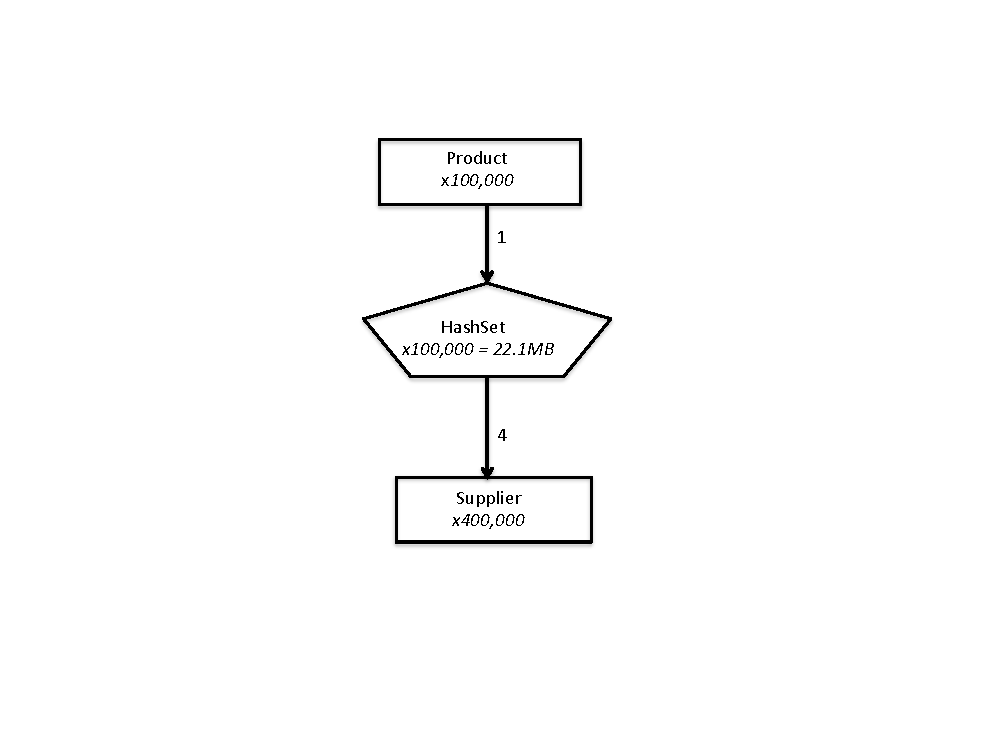
\includegraphics[width=.80\textwidth]{part1/Figures/collections/product-hashset.pdf}
 \caption{A relationship between products and alternate suppliers,
  stored as a
  \class{HashSets} of alternate \class{Suppliers} related to \class{Products}.}
  \label{fig:product-hashset}
\end{figure}


Using a \class{HashSet} for alternate suppliers turns out to be a
very costly decision. The alternate suppliers are represented by 100,000
very small \class{HashSet}s, each consuming 232 bytes, for a total cost of 22.1MB. 
This cost is all overhead.
It's hard to think of a good reason why such a heavy-weight collection should ever be used
 for storing just a few entries, and yet, this pattern is very, very common. For
 small sets, \class{ArrayList} is almost always a better choice. \class{HashSet} maintains uniqueness
  and provides fast access, but enforcing uniqueness
is not always needed. If uniqueness is
important, it can be enforced for an \class{ArrayList} 
 with  little extra checking code, and usually without significant performance
 loss when sets are small. Figure~\ref{fig:product-arraylist} shows improved
 memory usage with \class{ArrayList}. Each \class{ArrayList} incurs 80 bytes of overhead,
approximately a third the size of a \class{HashSet}.
 \begin{figure}
  \centering
 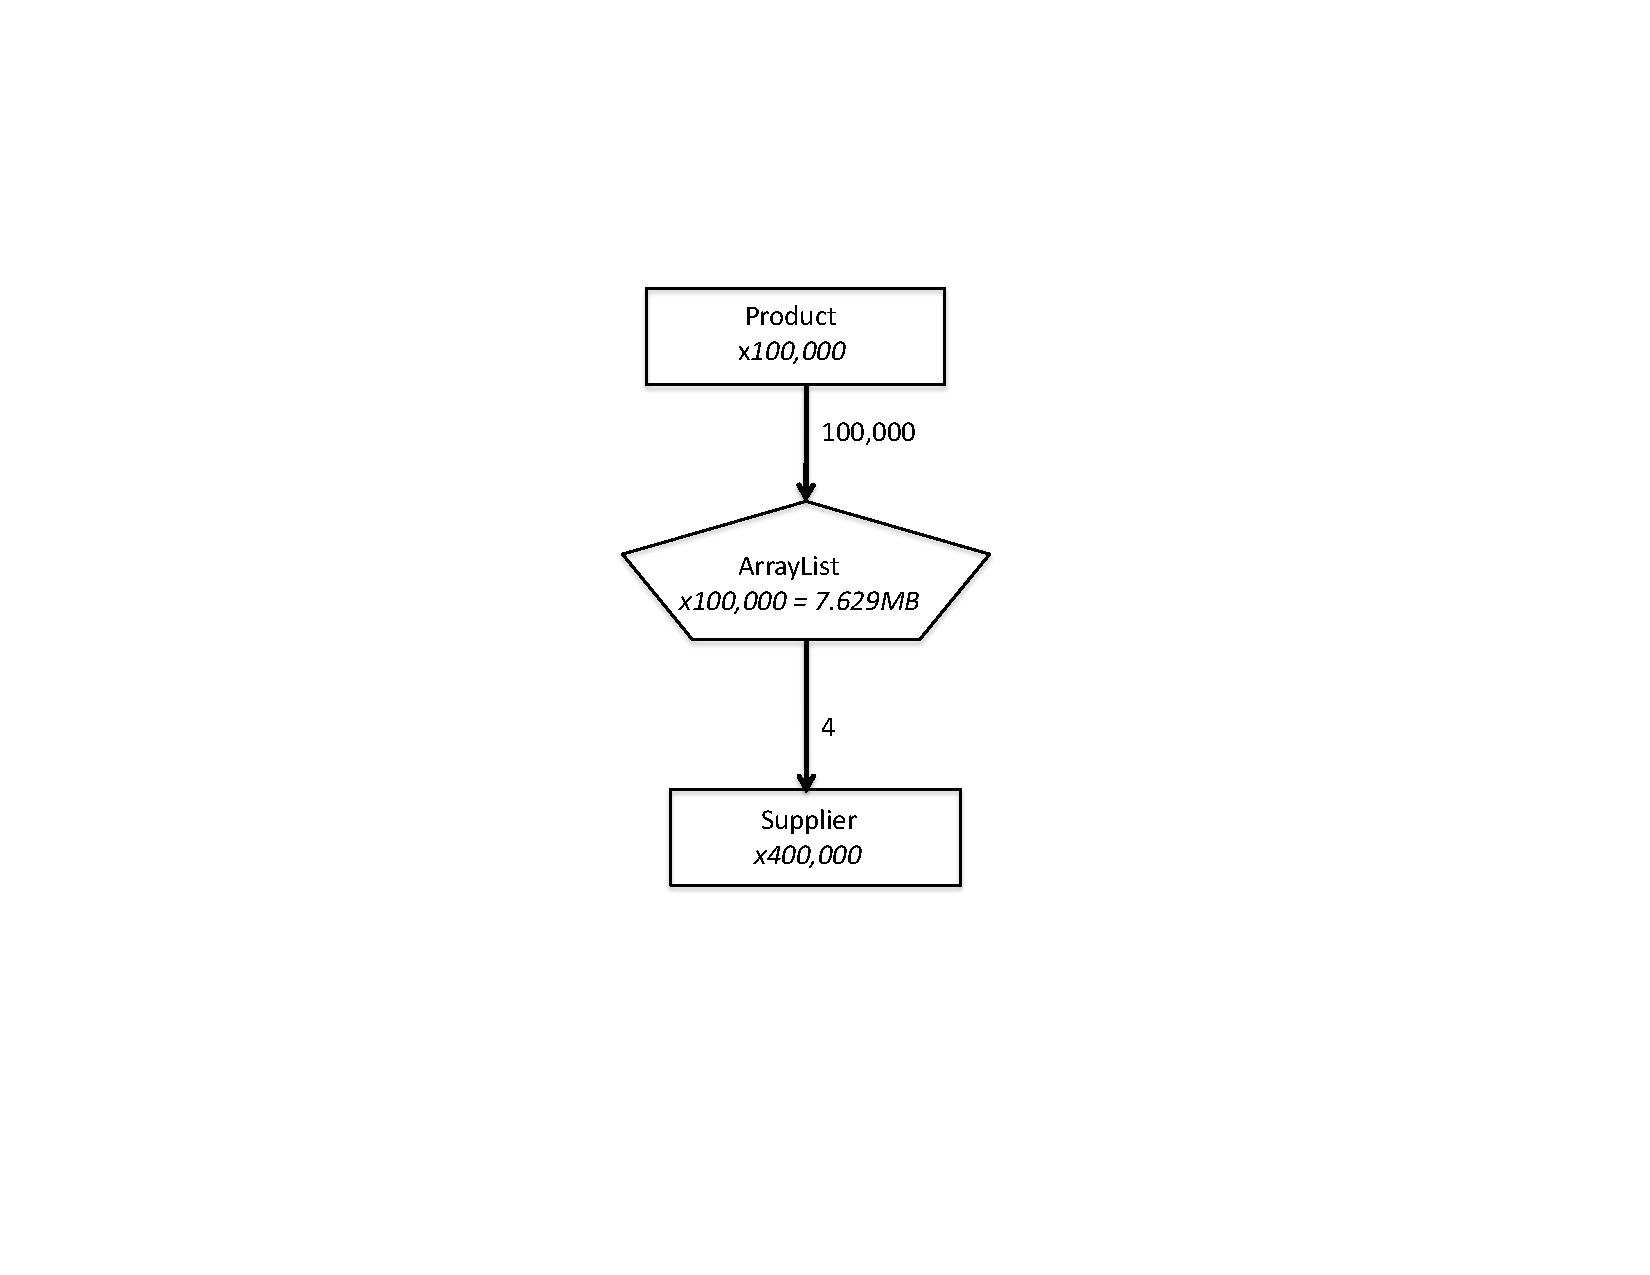
\includegraphics[width=.80\textwidth]{part1/Figures/collections/product-arraylist.pdf}
 \caption{A relationship between 100,000 products and alternate suppliers,
 where the alternate \class{Suppliers} associated with each \class{Product} are
 stored in an \class{ArrayLists}.}
  \label{fig:product-arraylist}
\end{figure}
This simple change saves 14.5MB. 


\section{Inside the Collections}
\label{sec:collectioncost}
Let's look inside a \class{HashSet} to see why it is so much bigger than an
\class{ArrayList}. Some of its extra cost is because of additional functionality,
such as providing uniqueness checking and entry removal in constant time.
\class{HashSet} is also optimized for performance, and sacrifices memory 
under the assumption that \class{HashSet}s will contain a large number of
elements. Additionally, \class{HashSet} delegates its work to a
degenerate \class{HashMap}, that is, one with keys but no values. This decision,
to reuse the more general \class{HashMap} code, adds to the memory
cost. Other extra costs are due to unavoidable Java overhead.

The internal structure of a \class{HashSet} is shown in
Figure~\ref{fig:inside-hashset}. All
collections are similar in their basic structure: a wrapper which remains
stable, and an internal structure that changes as entries are added and removed.
 \begin{figure}
  \centering
 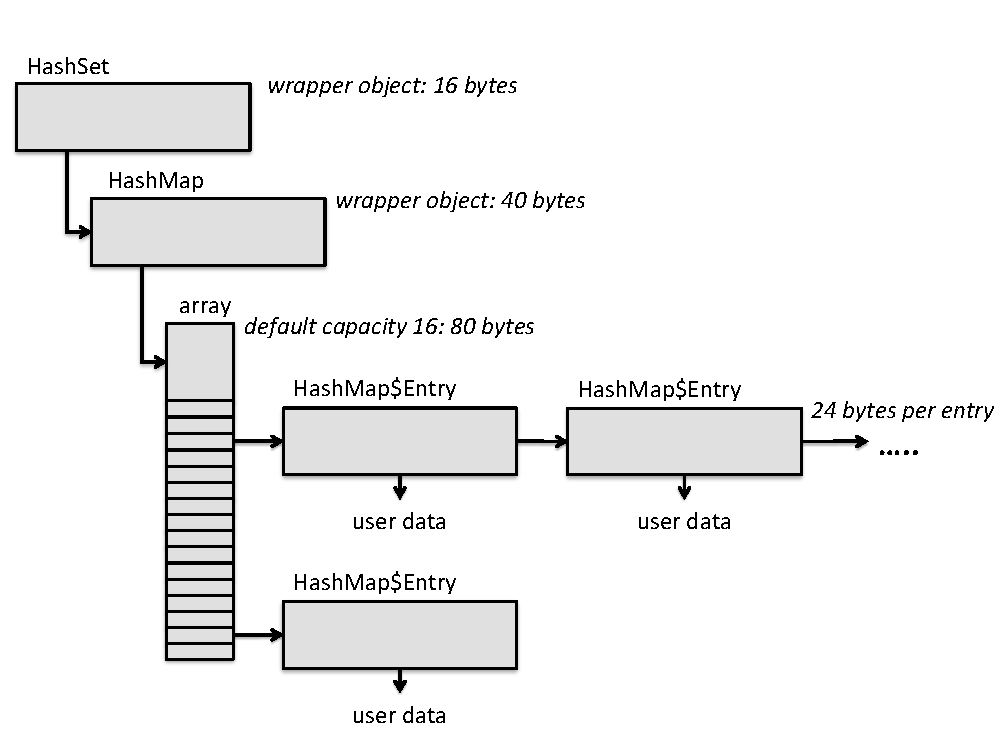
\includegraphics[width=.80\textwidth]{part1/Figures/collections/inside-hashset.pdf}
  \caption{The internal structure of a \class{HashSet}, shown with 3 entries.}
  \label{fig:inside-hashset}
\end{figure}


\begin{description}
\item[Wrappers] The \class{HashSet} object itself is just a wrapper,
delegating all of its work to a \class{HashMap}. Therefore, there is an additional wrapper,
a \class{HashMap} object. All
collections have wrapper objects, but a \class{HashSet} has two of them. 
Together they incur a fixed cost of 56 bytes.
 
\item[Internal structure] \class{HashMap} uses a \emph{chaining} design. There
is an array of hash buckets, where each slot points to a linked list of
\class{HashMap\$Entry} objects that map to the same
hash bucket. The default initial capacity is 16, to allow for growth.
Including its JVM overhead, the array adds a fixed cost of 80 bytes.
 
\class{HashMap} maintains a
\class{HashMap\$Entry} object for each element stored in the collection. 
These cost 24 bytes each. Note that since this is a
\class{HashSet}, the value field in each \class{HashMap\$Entry} object is not
used\footnote{There is an additional memory cost that occurs in a very common
case: if you choose to iterate over the contents of the set.
The first time you create an iterator, a 16-byte \class{HashMap\$KeySet} object will be created and retained for the lifetime of the set. This cost is not reflected in any of
our diagrams or numbers.}.
\end{description}

In contrast, \class{ArrayList} is a simpler structure, as shown in
Figure~\ref{fig:inside-arraylist}. It's an expandable array,
consisting of a wrapper object, and an array that points directly at the data
elements. As a result, it has a smaller fixed cost and a smaller
variable cost than \class{HashSet}. Fixed costs
include wrappers and the array's JVM overhead, and empty slots.
The fact that \class{HashSet} delegates to \class{HashMap} inflates its fixed cost. 
Lower fixed cost means that an \class{ArrayList} with just a few
 elements is smaller than a \class{HashSet} with the same elements. 
The variable cost of an \class{ArrayList} is a slot in the array, which
is 4 bytes. The variable cost of a \class{HashSet} is an
entry array pointer plus a \class{HashMap\$Entry}, which is 28 bytes. Lower variable cost means that
 \class{ArrayList} scales much better than \class{HashSet}. So \class{ArrayList} is better
 both for small and large sets.
 \begin{figure}
  \centering
 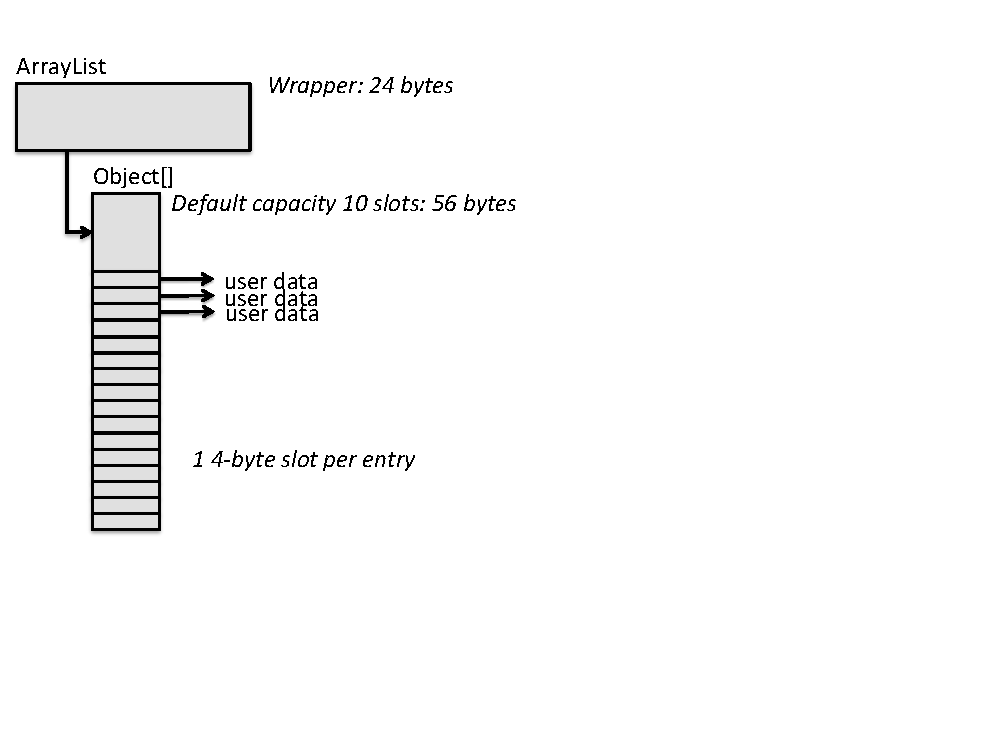
\includegraphics[width=.80\textwidth]{part1/Figures/collections/inside-arraylist.pdf}
 \caption{The internal structure of an \class{ArrayList}, shown with three
 entries and default capacity. \class{ArrayList} has a relatively low
 fixed overhead, and is scalable.}
  \label{fig:inside-arraylist}
\end{figure}
 

Table~\ref{tab:small-collection-costs} shows the memory costs of four basic
collections, \class{ArrayList}, \class{LinkedList}, \class{HashMap}, and \class{HashSet}.
This table shows the default size when the collection is just allocated without
entries, and any additional entry cost. These costs have
been calculated based on the Sun JVM, using the techniques described in Chapter~\ref{chapter:delegation}. 
The various other Java standard
library implementations in circulation have costs
similar to these. You can calculate them using the same methodology.


\begin{table}
\centering
 		\begin{tabular}{lcc}
 		\toprule
	 	 Collection & \multicolumn{2}{c}{Size in bytes} \\
	 	 & with 4 entries & with n entries \\
	 	 \midrule
	 	ArrayList & 80 & 80 , n = 0 .. 10 \\
 		LinkedList & 144 & 48 + n*24 , for any n \\
 		HashMap & 216 & 120 + n*24 , n = 0 .. 11 \\
 		HashSet & 232 & 136 + n*24 , n = 0 .. 11 \\
	 	\bottomrule
	 	\end{tabular}
	 	
%	\caption{}\label{tab:small-collections-default}{}
 		\begin{tabular}{lcc}
 		\toprule
	 	 Collection & \multicolumn{2}{c}{Size in bytes} \\
	 	 & with 4 entries & with n entries \\
	 	 \midrule
	 	ArrayList & 56 & 40 + (n/2)*8 , n = 0 .. 10 \\
 		LinkedList & 144 & 48 + n*24 , for any n\\
 		HashMap & 184 & 88 + n*24 , n = 0 .. 5 \\
 		HashSet & 200 & 104 + n*24 , n = 0 .. 5 \\
	 	\bottomrule
 	 	\end{tabular}
%	\caption{}\label{tab:small-collections-minimum}{}
	\caption{Size in bytes of some common collection classes, when they contain very few
	elements. n = number of elements. Formulas are valid only for the range specified. (a) Default size
	(b) Minimum size.[TODO: format as a table with two subtables; footnote re: doesn't include KeySet]}
	\label{tab:small-collection-costs}
\end{table}

Our guess is that the
collection class developers would be surprised by the relationship usage pattern
that results in hundreds of thousands of small \class{HashSets}. Why bother
implementing expandable structures and clever hashing algorithms for only a few entries?
This mismatch between collection implementation and usage is 
a leading cause of memory bloat. The overhead cost of a \class{HashSet} is
remarkably high. Creating many small collections multiplies this basic infrastructure
cost, which is all overhead, filling the heap. 
 

\section{Properly Sizing Collections}
\label{sec:proper-size}

Collections such as \class{HashMap} and \class{ArrayList} store their entries in
arrays. When these arrays become full, a larger array is allocated
and the entries are copied into the new array.  Since allocation and copying
can be expensive, these entry arrays are always allocated with some extra
capacity, to avoid paying these growth costs too often. 
This is why the initial capacity of an \class{ArrayList} is 10 rather than zero
 or one, and why its capacity increases by
50\% when it is reallocated. 
Similarly, the capacity of a \class{HashMap} starts at 16, and grows by a
factor of 2 when the \class{HashMap} becomes 75\% full. 

These default policies trade space
for time, on the assumption that collections grow. However,
collections used to represent relationships may have hundreds of thousands of
small collections that don't grow. As a result, there is no performance gain, and the extra
empty array slots can add up to significant bloat problem, unless you take
explicit action.

 Fortunately, it is possible to right-size
 \class{ArrayLists}. If you know that an \class{ArrayList} has a maximum size
 $x$, which is less than the default size, then it's worth passing $x$ as a
 parameter to the constructor to set the initial capacity of the
 \class{ArrayList} to $x$. However, if you are wrong and the \class{ArrayList}
 grows bigger than $x$, then it will grow by 50\%, which may
 be worse than just taking the default initial size.
 
 Alternatively, you can call the \code{trimToSize} method which shrinks the
 entry array by eliminating the extra growth space. Trimming reallocates and
 copies the array, so it is expensive to keep calling \code{trimToSize} while an
 \class{ArrayList} is still growing. Trimming is appropriate after
 it has been fully constructed and will never grow again. In fact, applications
 often have a build phase followed by a used phase, in which case
 \class{ArrayLists} can be trimmed between these two phases, so that the cost of reallocation 
 and copying is paid only once.
 
 Returning to the example of the relationship between products and alternate
 suppliers, the \class{ArrayLists} in Figure~\ref{fig:product-arraylist} have
  default capacity. If we assume that the the relationship is built in one
  phase, and used in another phase, then it is possible to trim the
  \class{ArrayLists} after the first phase. This should save quite a bit of
  space, since there are 100,000 \class{ArrayLists} with four entries on
  average. In fact, trimming these
 \class{ArrayLists} saves 2.3MB, or another 30\%, as shown in
 Figure~\ref{fig:trimmed-product}. 

 \begin{figure}
  \centering
 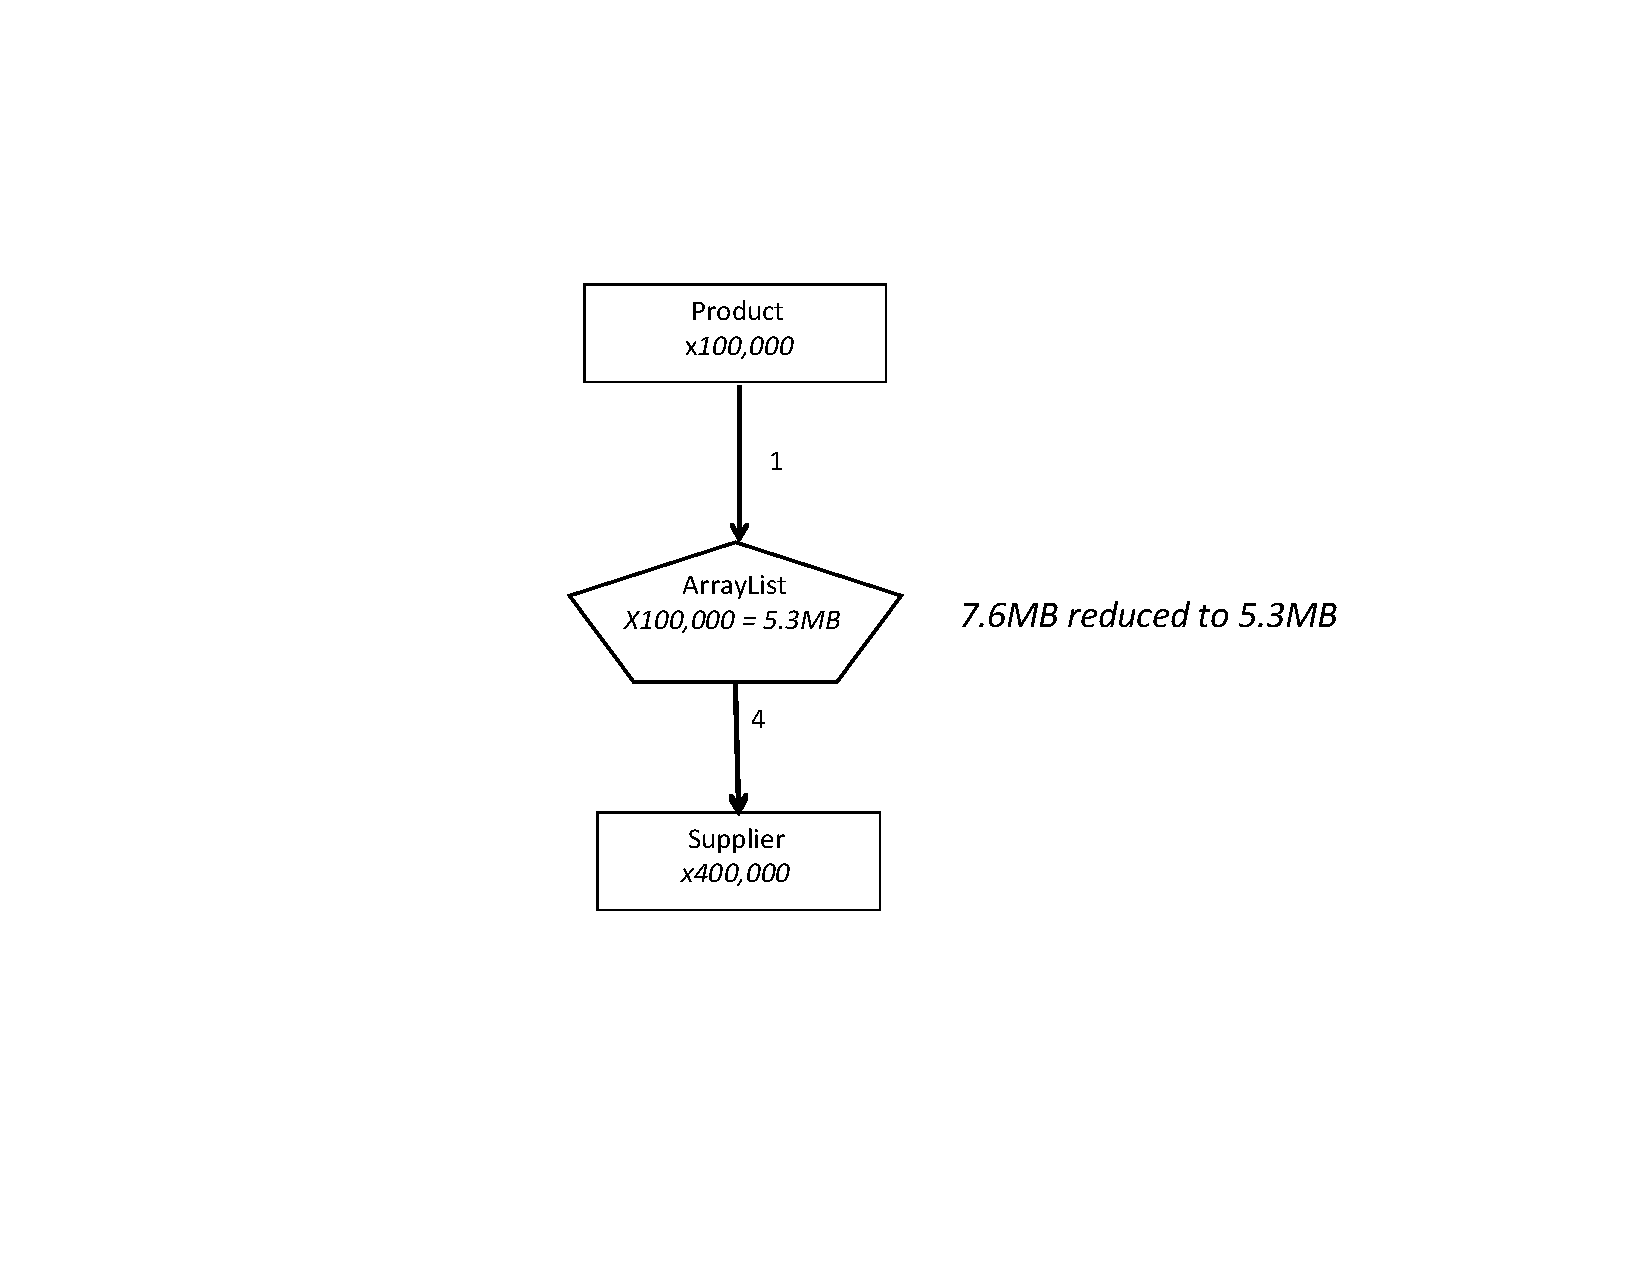
\includegraphics[width=.80\textwidth]{part1/Figures/collections/trimmed-product.pdf}
 \caption{The relationship between \class{Product}s and \class{Supplier}s after
 all of the
 \class{ArrayLists} have been trimmed by calling the \code{trimToSize} method.}
  \label{fig:trimmed-product}
\end{figure}
 
\class{HashSets} and \class{HashMaps} do not have \code{trimToSize} methods,
but it is possible to pass the initial capacity and load factor as constructor
parameters when creating a \class{HashSet} or \class{HashMap}. 
However, before changing the initial capacity, you should
ask yourself whether using a \class{HashSet} or \class{HashMap} is a
wise decision in the first place. If you are going to end up with many
collections with fewer than 16 elements, perhaps there is a more memory-efficient solution, like
\class{ArrayList}.
  
A \class{LinkedList} is another alternative for small collections, and are
better than \class{ArrayLists} if the collections are changing a lot. The
24 byte per-entry cost is larger, but there is no element array, and only one
extra entry, which is a sentinal.

\section{Avoiding Empty Collections}

Too many empty collections is another common problem that leads to memory bloat.
A quick look inside an empty collection shows that it is not all that empty. 

bytes, assuming a default initial size. 
Even if the default initial size is overridden and set to zero, empty
collections are still large. A zero-sized \class{HashMap} consumes 56 bytes, and a zero-sized
\class{ArrayList} consumes 40 bytes. Empty \class{HashSets} are even bigger.

Empty collection problems are generally caused by eager initialization, that is,
allocating collections before they are actually needed. Exacerbating this
problem, collections themselves also allocate their internal objects in an eager
fashion. For example, \class{HashMap} allocates its entry array before any entries are inserted.
You might think that eager initialization is not such a big problem, since
entries will be added eventually. However, often collections are allocated
just in case they are needed later, and remain empty throughout the execution.

Suppose the relationship
in Figure~\ref{fig:trimmed-product} is initialized by the code:
\begin{shortlisting}
List<Product> products;
int numProducts;
   ..
   public void initAlternateSupplierRelationship() {
       ..
       for (int i = 0; i < numProducts; i++) {
          Product product = products.get(i);
          product.alternateSuppliers = 
                           new ArrayList<Supplier>();
       }
   }
\end{shortlisting}
Initially, each product is mapped to an empty \class{ArrayList} for alternate
suppliers, so there are 100,000 empty \class{ArrayLists} before any
\class{Supplier}s are inserted. As the alternate suppliers are populated, many
of these \class{ArrayLists} will become non-empty, but it is likely that a good
number of products have no alternate suppliers. If 25\% of the products in the
final graph still have no alternate suppliers, there will be 25,000 empty
\class{ArrayLists}, which consume about 1MB even after calling
\code{trimToSize}.
Figure~\ref{fig:empty-array} shows the entity-collection
diagram after removing 25,000 empty alternate supplier \class{ArrayList}s. Note
that there are now only 75,000 alternate supplier \class{ArrayList}s shown,
since there are no more empty \class{ArrayList}s. Therefore, we adjust the
average fanout in and out of \class{ArrayList} to .75 and
5.33 respectively.
\begin{figure}
  \centering
 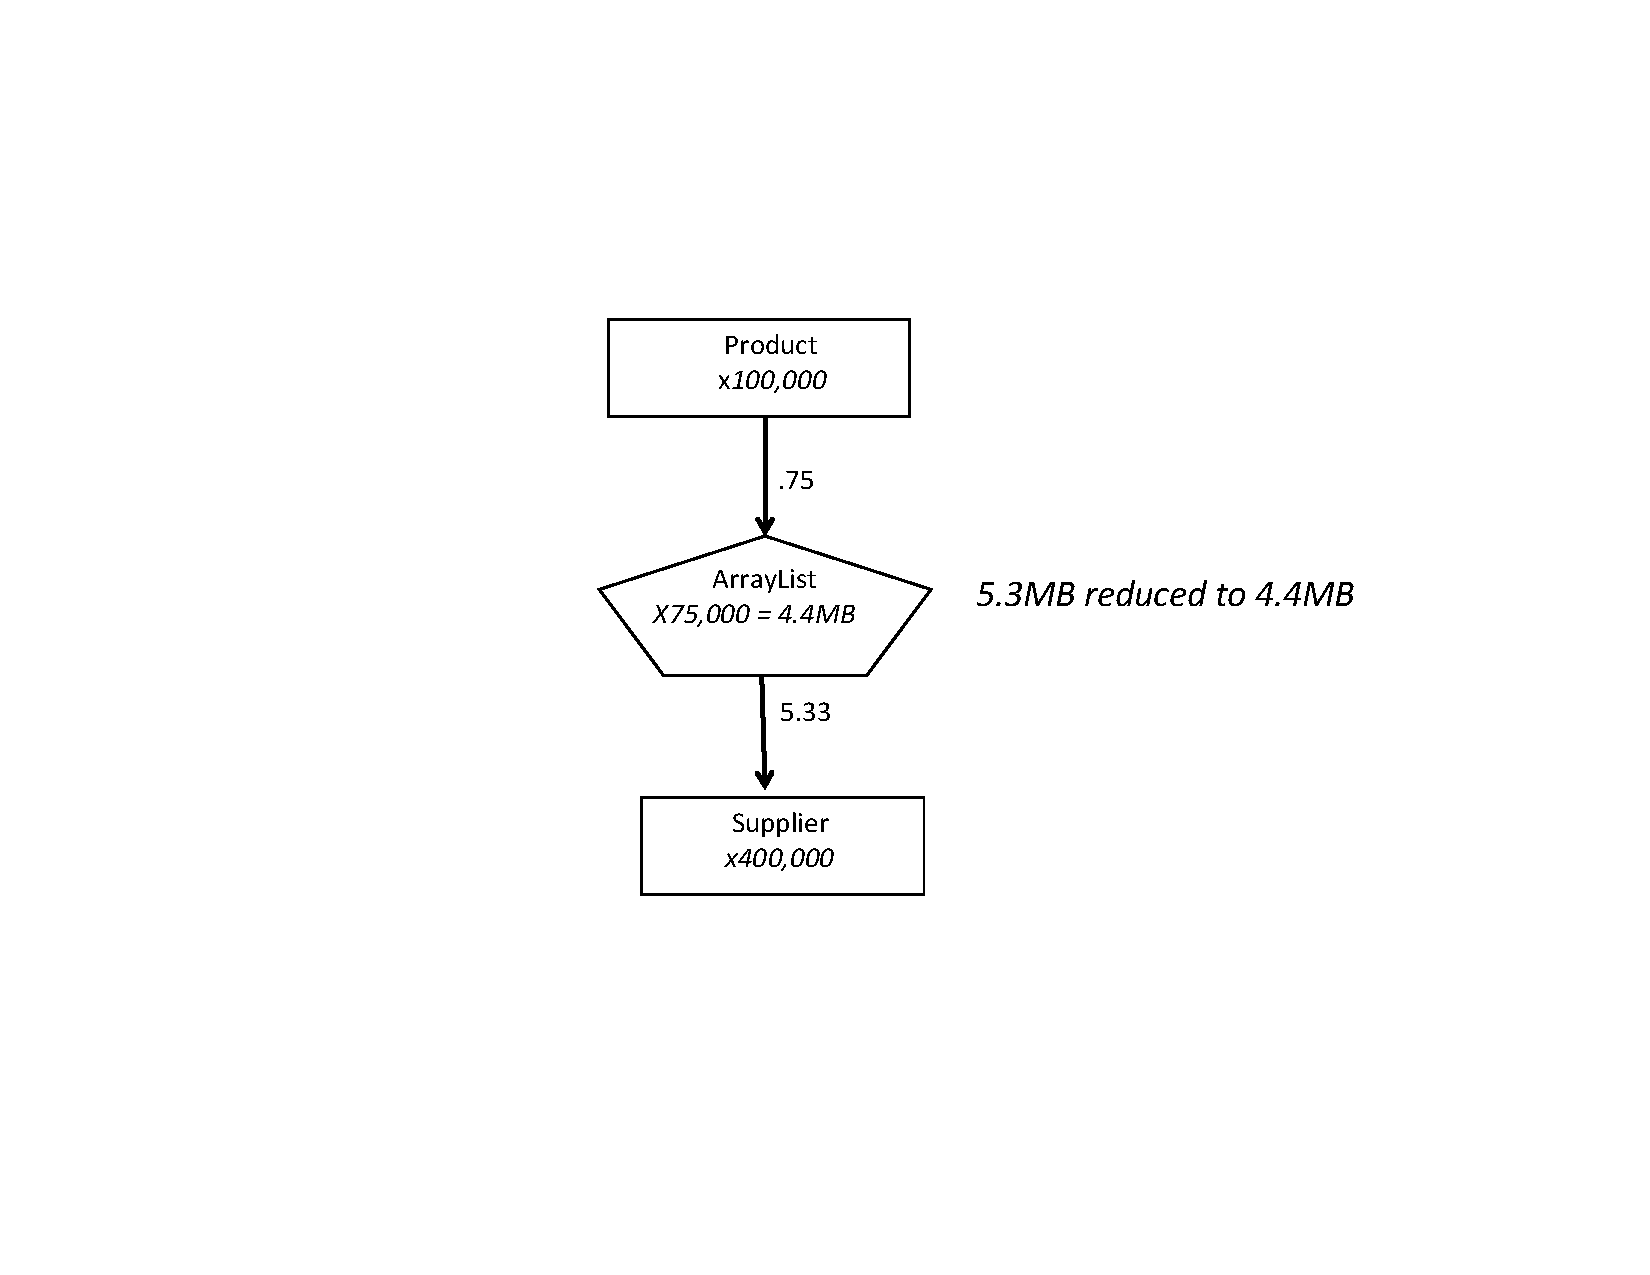
\includegraphics[width=.80\textwidth]{part1/Figures/collections/empty-product.pdf}
 \caption{The relationship between \class{Product}s and \class{Supplier}s
  where there are no empty \class{ArrayLists}.}
  \label{fig:empty-array}
\end{figure}
 
 Delaying allocation prevents creating too many empty collections.
 That is, instead of initializing all of the collections that you think you
 may need, allocate them on-demand, just before inserting an edge. On-demand
 allocation requires more checking code, to avoid \code{NullPointerException}s.
 
 Alternatively, you can initialize collection fields to reference static empty collections,
 including EMPTY\_SET,
 EMPTY\_LIST, and EMPTY\_MAP. For example, 
 calling static method \code{Colletions.emptyList} to initialize edge
 \class{ArrayLists} maps all nodes to a singleton immutable static
 \class{ArrayList}, so that no empty \class{ArrayLists} are created:
 \begin{shortlisting}
     public void initAlternateSupplierRelationship() {
       ..
       for (int i = 0; i < numProducts; i++) {
          Product product = products.get(i);
          product.alternateSuppliers = 
                               Collections.emptyList();
       }
     } 
 \end{shortlisting}
This initialization avoids the need to check whether an \class{ArrayList}
exists at every use. For example, the size method and iterators will just work.
However, you have to be careful not to let any references to static empty
collections escape their immediate context. 
If you give out a reference to a static empty collection, 
then there is no way to update this escaped empty-collection reference
once an actual collection is allocated. 

\section{Fixed Size Collections}

Java collections can grow to be
arbitrarily big, but this functionality comes at a cost.
Collections include wrapper objects, and 
may be sized with extra growth room. If
you know that the size of a collection is fixed, having the ability to expand
the collection is unnecessary, and it is better to choose a cheaper alternative.
In fact, often you can use a
simple Java array, and not use a collection at all.  

In our example, alternate suppliers are stored in an
 \class{ArrayList}, which inside is a
wrapper pointing to an array of \class{Suppliers}.  If we assume that
every product has at most four alternate suppliers, then  it isn't 
necessary to store these in an \class{ArrayList} --- a simple array will do.
Eliminating the \class{ArrayList} object removes 24 bytes per
product, but we have to add 4 bytes to each \class{Product} to store the number
of alternate suppliers. The total savings is 1.43MB for 75,000 products:
\begin{shortlisting} 
class Product {
	String sku;
	String name;
	.. 
	int numAlternateSuppliers;
	Supplier[4] alternateSuppliers;
}
\end{shortlisting}
 

%\begin{figure}
 % \centering
% 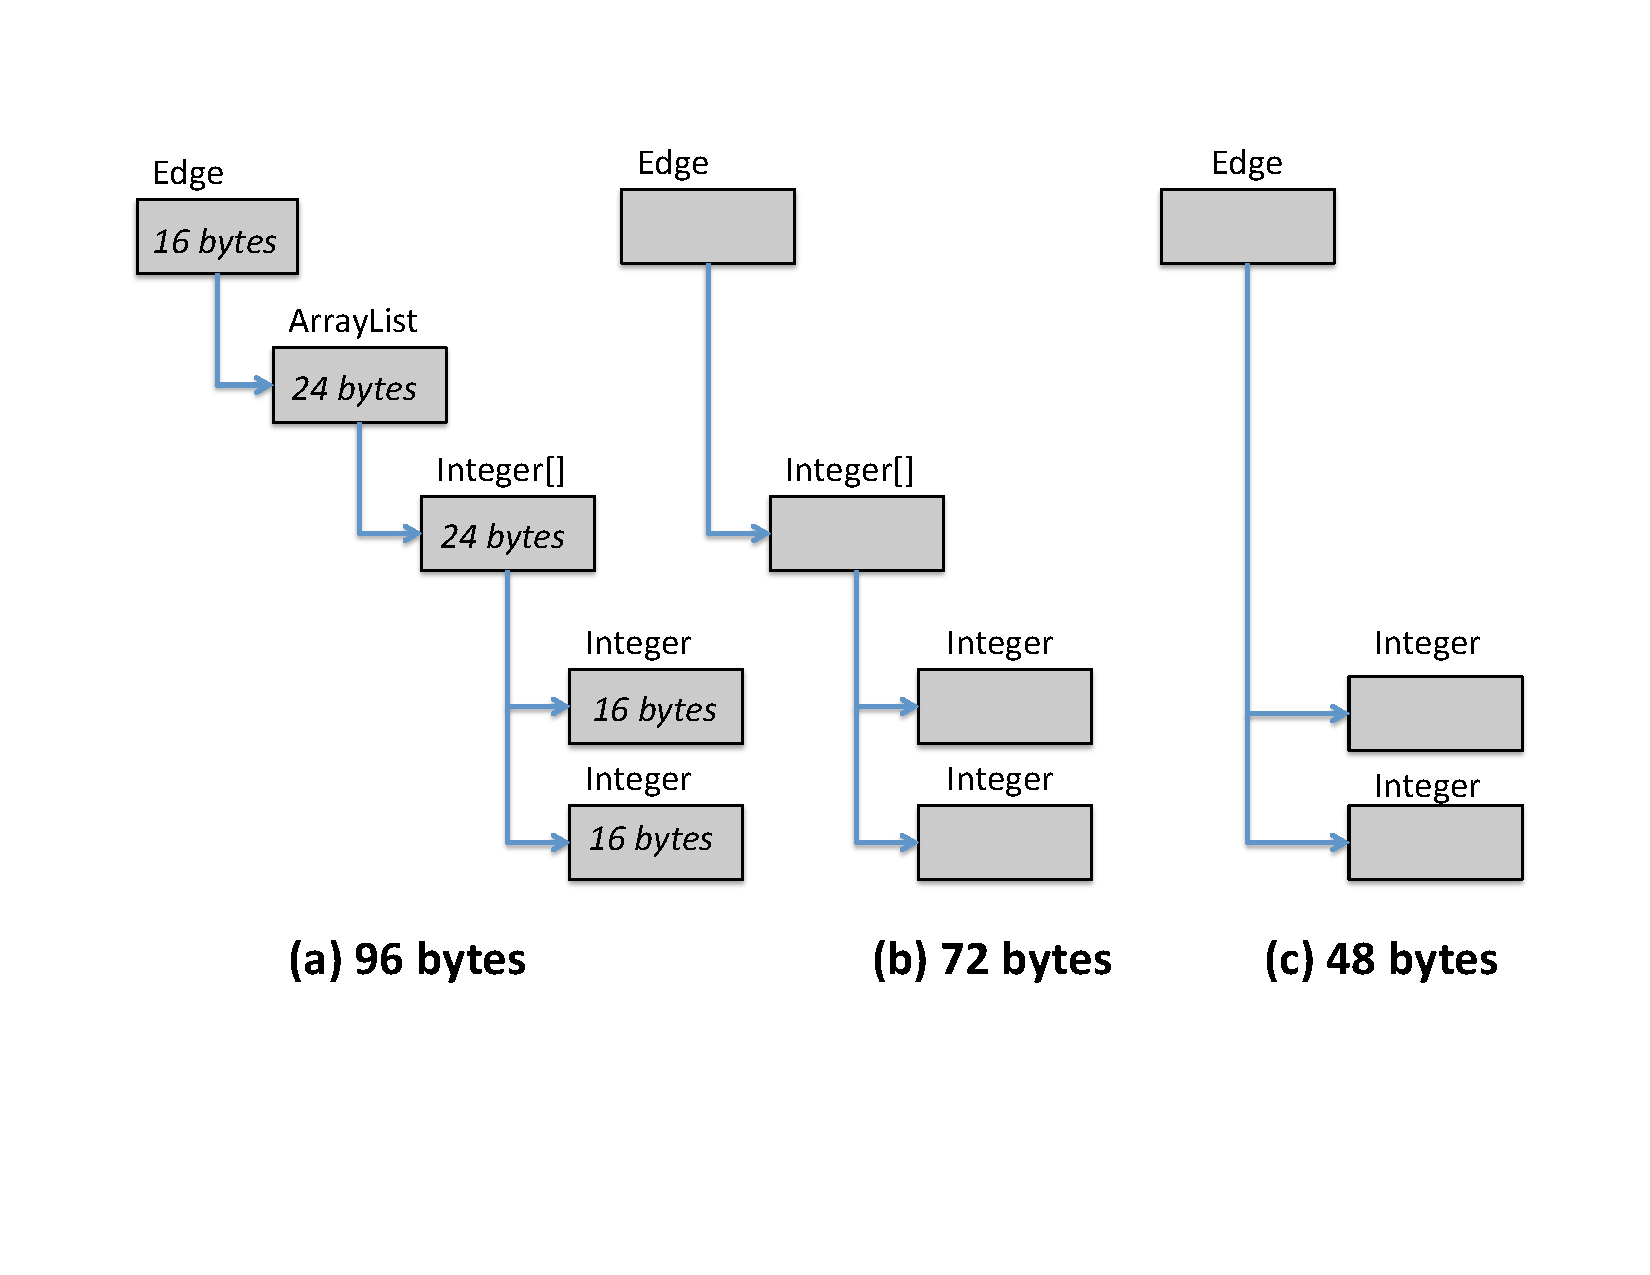
\includegraphics[width=.80\textwidth]{part1/Figures/collections/Edges.pdf}
%  \caption{(a) An \class{Edge} has 96 bytes. (b) Replacing the
%  \class{ArrayList} by an array eliminates 24 bytes. (c) Inlining the array
%  eliminates another 24 bytes.}
%  \label{fig:edges}
%\end{figure}
This is an example of choosing an overly-general collection. In
this situation, you don't need a collection at all. Using \class{ArrayList}
for storing fixed- or bounded-size arrays is a
common practice that can be easily avoided.

There is one final optimization that can be performed on the \class{Product}
class. Namely, making the four alternate suppliers into fields of
\class{Product} instead of elements of an array. This optimization
 a 32 byte array object for 75,000 products, while adding three additional
 fields to the \class{Product} for 100,000 objects, saving another 1.1MB in
 total:
\begin{shortlisting}
class Product {
	String sku;
	String name;
	.. 
	Supplier alternateSupplier1;
	Supplier alternateSupplier2;
	Supplier alternateSupplier3;
	Supplier alternateSupplier4;
}
\end{shortlisting}

This representation is very similiar to the original \class{Product} class in
section~\ref{sec:rarely-used} where there is one alternate suppler field, and
here there are four. Taking all of the optimizations 
together, we have gone from the initial \class{HashSet} representation
of 22.1MB in Section~\ref{section:choosing-collection} to the in-lined field
representation of 1.86MB. 

\section{Hybrid Representations}

An interesting case is when the sizes of the collections used in a relationship
is not uniform. That is, some collections are small and some collections are
very big.  It's reasonable to use an expensive collection like \class{HashSet}
for the big collections, but then the small collections pay the price. One way
to handle this problem is to use a hybrid representation. For example, you can
use arrays for smaller collections, and \class{HashSets} for larger
collections. 

One catch is that usually you will not know in advance which collections in the
relationship will end up being small and which will grow to be large. Therefore
a conversion operation will be necessary at some point if a collection grows
large enough. Each collection starts as an array, and then once it
grows past a threshhold, it is converted to a \class{HashSet}.

In our example, suppose that the vast majority of products have four alternate
suppliers on average, but a few products have over 100 alternate suppliers. We
can choose a threshhold, say six entries, which triggers a conversion to a
\class{HashSet} when the threshhold is exceeded. Here is the class
\class{Product}:

\begin{shortlisting} 
public class Product {

	    static final int threshhold = 6;
		String sku;
		String name;
		..
		int numAlternateSuppliers;
		Supplier[] alternateSuppliers;
		HashSet<Supplier> bigAlternateSuppliers;
		
		void addAlternateSupplier(Supplier supplier) {
		
		    /* Check for duplication */
		    if (hasAlternateSupplier(supplier)) {
		         return;
		    }
		
		    /* Try to add the supplier to the array alternateSuppliers */
		    if (numAlternateSuppliers == 0) {
		        alternateSuppliers = new Supplier[threshhold];
		    }
			if (numAlternateSuppliers < threshhold) {
			    alternateSuppliers[numAlternateSuppliers++] = supplier;
			    return;
			}
			
			/* If threshhold is exceeded, need to use bigAlternateSuppliers */
			if (numAlternateSuppliers == threshhold) {
			    bigAlternateSuppliers = new HashSet<Supplier>();
			    for (int i = 0; i < threshhold; i++) {
			    	bigAlternateSuppliers.add(alternateSuppliers[i]);
			    }
			    alternateSuppliers = null;
			}
			bigAlternateSuppliers.add(supplier);
			numAlternateSuppliers++;
			return;
		}
}
\end{shortlisting}
The method \code{addAlternateSupplier} adds the supplier to the array if the
size is less than the thresshold, otherwise, it adds the supplier to the \class{HashSet}.
It allocates the alternate supplier array and \class{HashSet} 
only if and when it is needed, to avoid wasting space with empty collections
when there are no or only a few alternate suppliers.

Implementing hybrid representations is more complicated than just using one
collection for a relationship. However, it can save significant space in some
cases.

\section{Summary}

Collections used to represent relationships often result in many small
collection instances, whose cost is dominated by a fixed-size
overhead. This chapter describes a number of ways to mitigate high fixed memory
costs for relationships implemented with collections:
\begin{itemize}
  \item Choose the most memory-efficient collection for the job at hand. In
  particular when collections have at most a few elements in them, you don't
  need expensive functionality like hashing. 
  \item Make sure collections are properly sized. If you know that a collection
  will not grow any more, then there is no reason to maintain extra room for
  growth.
  \item Avoid lots of empty collections. It is common to allocate collections 
 ahead of time, whether or not they will eventually ever be used. If you
 postpone creating them until they are needed, often you will end up with fewer collections, 
 and no empty collections.
 \item Use arrays instead of \class{ArrayLists} when you know the maximum size
 of the collections in advance. You can also eliminate an
 \class{ArrayList} altogether when there are always at most a few entries that
 can be stored in fields.
 \item When the usage pattern is not uniform, it is sometimes reasonable to use
 a hybrid representation.
\end{itemize}
Knowing which relationships and collections in your application are the most
important and need to scale is key to applying these optimizations effectively.  




